\subsection{Diffusion Transformer (DiT)}
\label{appendix:diffusion_transformer}

\begin{figure}
    \centering
    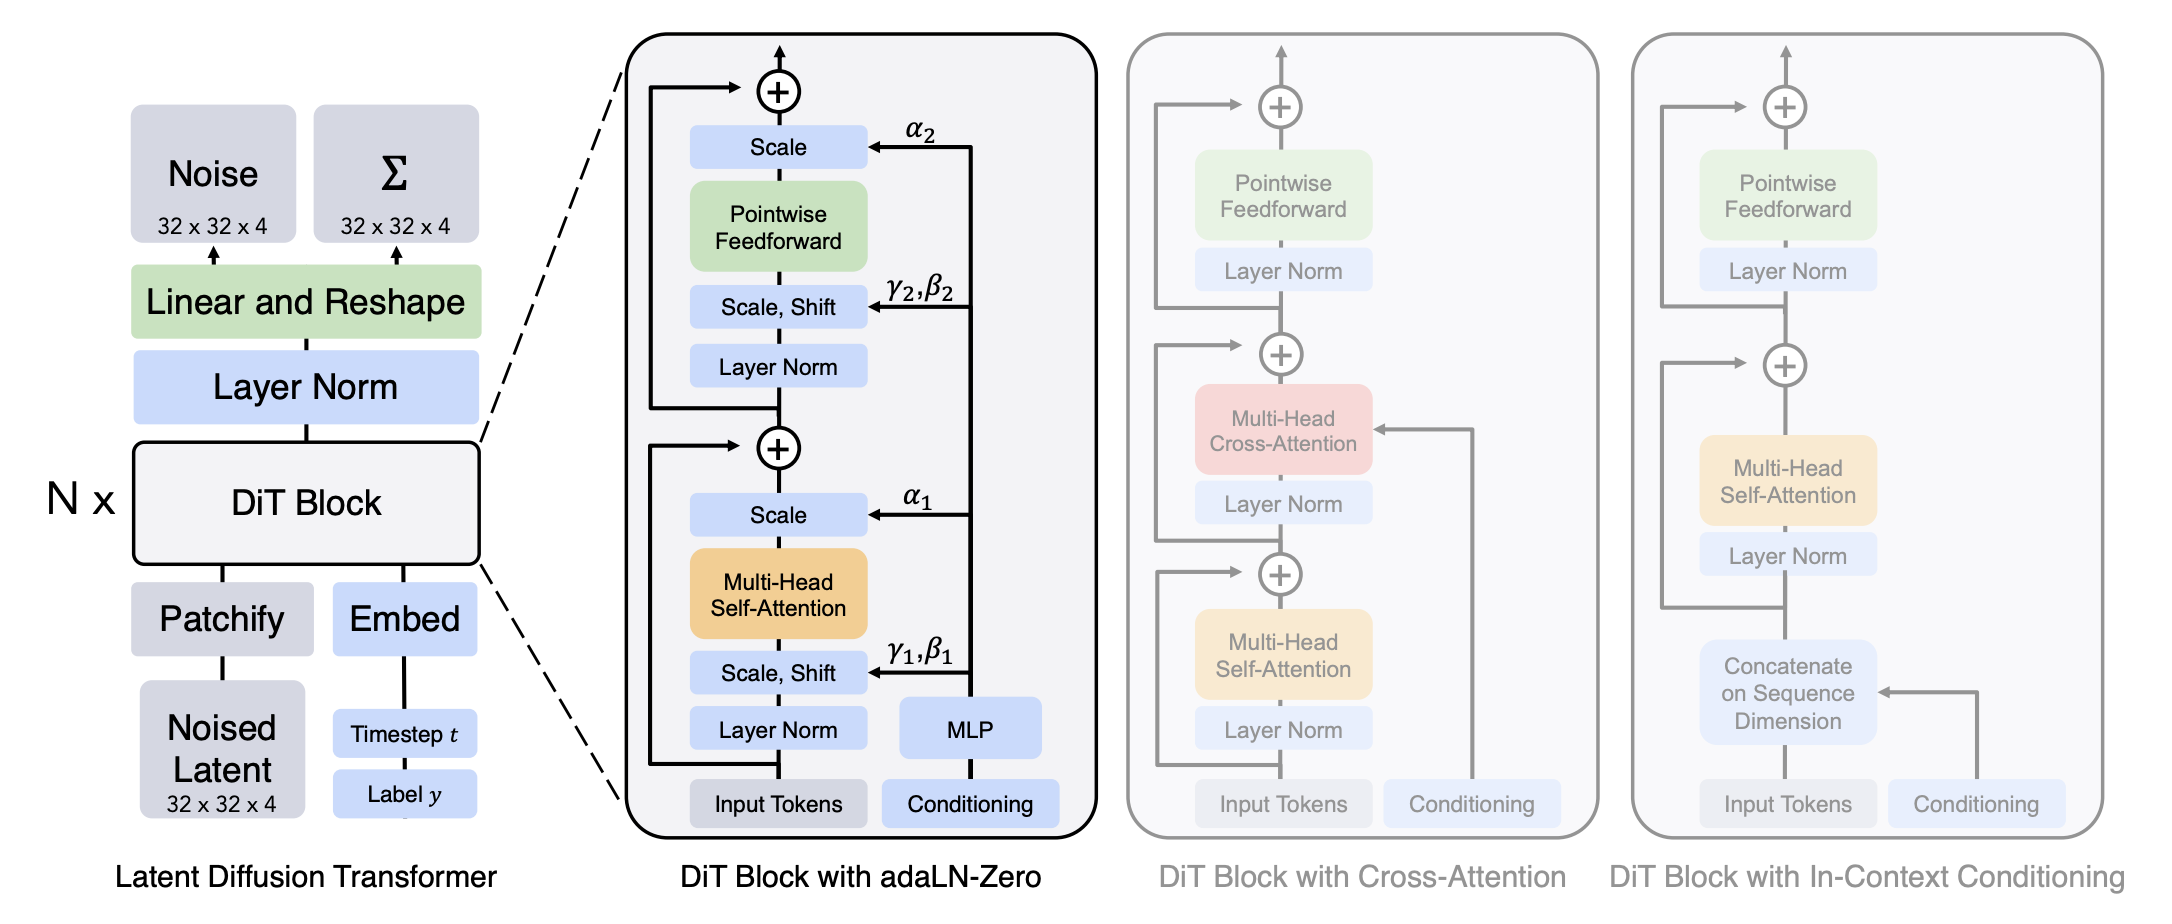
\includegraphics[width=0.8\textwidth]{images/appendix/diffusion_transformer/architecture.png}
    \caption{Diffusion Transformer (DiT) architecture \cite{diffusion_transformer}. On the right we see three DiT blocks: with adaLN (adaptive layer normalization, appendix \ref{appendix:blocks_norm}), with cross-attention, and with in-context conditioning. The transformer outputs noise prediction and diagonal covariance matrix.}
    \label{fig:diffusion_transformer_architecture}
\end{figure}

Diffusion Transformer (DiT) was introduced in a 2023 paper \cite{diffusion_transformer}. This paper explored new class of diffusion models based on transformer architecture. The researchers showed that the U-Net in Latent Diffusion Models (LDMs) can be replaced by a transformer, which also denoises the latents. Due to the scalability of transformers, they showed that this architectural change provides significant benefit to Gflops (giga floating point operations per second, which measure computational complexity of the model) and increases sample quality. In the paper the main task of DiT was to generate images on ImageNet and they achieved new best FID score of 2.27.

They take inspiration from Vision Transformer \cite{vision_transformer} (appendix \ref{appendix:vision_transformer}) paper where the image is first patchified (patches of size $p \times p \times 3$), turned into sequence of $T$ tokens, each with dimension $d$, positional embeddings are added (sinusoidal encoding), and then they feed this input to the DiT block, similar to how ViT operates.

\textbf{In-context conditioning block:} In order to add class label information and diffusion time embeddings (conditions), they just added these conditioning tokens to the input sequence. These tokens are similar to the case of \texttt{[CLS]} token in ViT (which was added at the beginning of the input sequence). After the final DiT block, they remove these tokens from the input, because they achieved the task of conditioning, and the transformer decoder can perform the noise prediction task.

\textbf{Cross-attention block:} In similar manner to Stable Diffusion, they use cross-attention with the class label $c$ and diffusion timestep embeddings $t$ and feed it into cross-attention, where the other input sequence (sequence of patch + position embeddings) is used as the query.

\textbf{Adaptive layer norm (adaLN) block:} adaLN normalization (appendix \ref{appendix:blocks_norm}) layers is another conditioning mechanism which adds the least Gflops to the model, which makes it the most compute-efficient.

\textbf{Noise prediction \& Diagonal covariance matrix:} The output of the model is learned noise prediction and a diagonal covariance matrix $\sum_\theta$ (shown in figure \ref{fig:diffusion_transformer_architecture}). We optimize $\sum_\theta$ in order to optimize the decoder $\mathcal{D}_{KL}$.

